  Les deux algorithmes implémentés ont un squelette très similaire ; il s'agit, à partir de la carte des profondeurs, de lier deux par deux les pixels de l'image générée puis de colorier chaque paire de la même couleur.

  Les deux algorithmes sont dotés d'une technique anti-surfaces cachées (implémentée différemment dans les deux cas). D'autre part, ils supportent tous deux l'utilisation de textures 
  
  \subsubsection{Algorithme de base (Witten, Inglis, Thimbleby)}

  Cet algorithme a été choisi pour sa simplicité qui le laisse tout de même fonctionnel ; il a été conçu à l'origine pour des autostéréogrammes aléatoires en noir et blanc (SIRDS) mais a été adapté ici à d'autres types de rendus.

  Les résultats obtenus sont cependant assez peu satisfaisants pour la représentation d'objets complexes, comme le montre la figure \ref{fig:autoste1} : l'image est assez plate, et l'objet en relief est fait de paliers superposés plutôt que d'avoir une surface lisse. De ce fait, représenter des détails ou des courbes est ardu. L'utilisation de textures peut permettre d'atténuer certains défauts visuels, mais pas de les effacer totalement.

\begin{figure}[h]
	\centering
	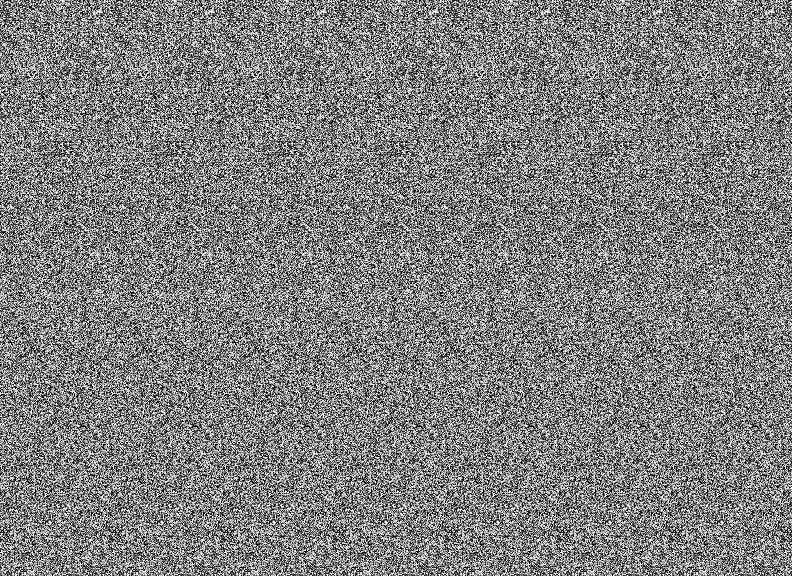
\includegraphics[scale=0.3]{autoste1.png}
	\caption{\label{fig:autoste1} Application d’une lumière diffuse à une sphère rouge \protect}
\end{figure}

  \subsubsection{Algorithme de W. A. Steer}
  
  L'algorithme de W. A. Steer a été choisi à cause des nombreuses améliorations qu'il apporte par rapport à l'algorithme précédent. En effet, il utilise une méthode de suréchantillonnage de l'image : dans une première étape, un autostéréogramme $n$ fois plus large que l'image de base est construit puis les pixels sont fusionnés par groupes de $n$. Ces étapes permettent d'améliorer la résolution en profondeur de l'autostéréogramme.
  
  Cet algorithme est plus lent que le précédent à cause du suréchantillonnage, mais les résultats obtenus sont nettement plus agréables à regarder car la résolution en profondeur est meilleure : l'image apparaît plus profonde comme le montre la figure \ref{fig:autoste2}. De plus, l'utilisation conjointe d'une texture et du suréchantillonage lisse l'image finale ; on n'y retrouve plus les ``paliers'' des résultats précédents. Ces paliers peuvent être visibles si le rendu choisi est de type aléatoire, mais ils sont beaucoup plus nombreux et rapprochés.

\begin{figure}[h]
	\centering
	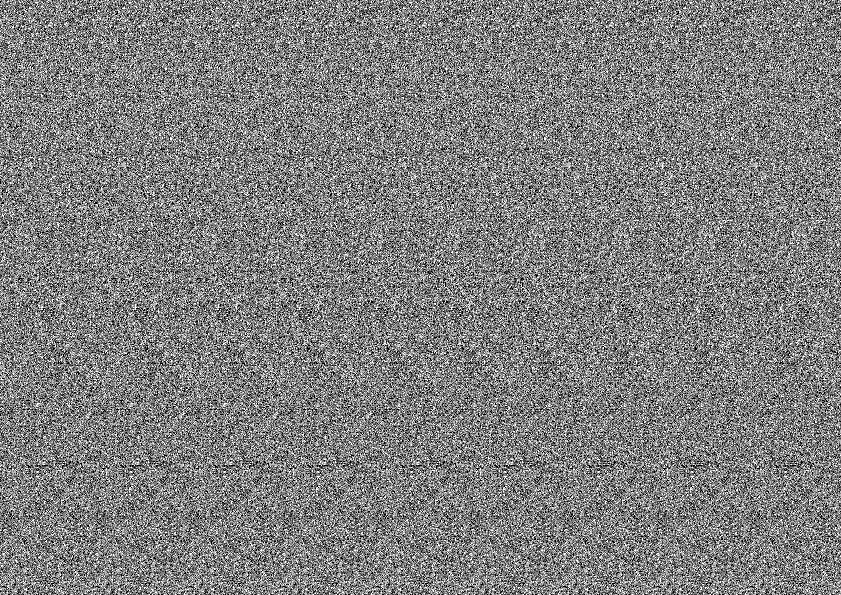
\includegraphics[scale=0.3]{autoste2.png}
	\caption{\label{fig:autoste2} Application d’une lumière diffuse à une sphère rouge \protect}
\end{figure}
